


\chapter{Boundaries and intersections}\label{chap:boundaries_and_intersections} 


\section{Introduction}

This chapter will derive various formulas that quantify the boundaries of the intersections. Many useful equations will be derived.


\section{The endpoints of path-volume intersections}\label{sec:endpoints_of_path_volume_intersect}

Consider an arbitrary multi-path \(\mathbf{J}\) and an arbitrary multi-volume \(U\). The intersection \(\mathbf{J} \cdot U\) is a multi-path, and the endpoints of this intersection are what will be sought: \(\nabla \bullet (\mathbf{J} \cdot U)\) 

Given an oriented path \(C\) and a volume \(\Omega\), there are two sources of endpoints for \(C \cdot \Omega\). The endpoints of \(C\) that happen to be inside of \(\Omega\) are also endpoints of \(C \cdot \Omega\). In addition, when \(C\) enters and exits \(\Omega\), this also creates endpoints for the intersection \(C \cdot \Omega\). When \(C\) enters \(\Omega\), \(C\) passes through the inwards oriented surface \(\nabla \Omega\) in the preferred direction. This intersection point, which has a weight of \(+1\), is a starting point for the intersection \(C \cdot \Omega\). When \(C\) leaves \(\Omega\), \(C\) passes through the inwards oriented surface \(\nabla \Omega\) in the opposite direction. This intersection point, which has a weight of \(-1\), is an ending point for the intersection \(C \cdot \Omega\).   

Consider a multi-path \(\mathbf{J}\) and a multi-volume \(U\). The endpoints of \(\mathbf{J}\) that are contained in \(U\), \((\nabla \bullet \mathbf{J}) \cdot U\), are endpoints of \(\mathbf{J} \cdot U\). In addition, the intersection of \(\mathbf{J}\) with the inwards oriented surface of \(U\), \(\mathbf{J} \bullet (\nabla U)\), also generates endpoints for \(\mathbf{J} \cdot U\). In total,  

\begin{thm}
\[\nabla \bullet (\mathbf{J} \cdot U) = (\nabla \bullet \mathbf{J}) \cdot U + \mathbf{J} \bullet (\nabla U)\]
\end{thm}

Below are examples of the endpoints of the intersection of a multi-path and a multi-volume. On the left, the multi-path and multi-volume is shown alongside the endpoints of the multi-path and the surface of the multi-volume. On the right, the intersection of the multi-path and multi-volume is shown alongside its endpoints.

\begin{center}
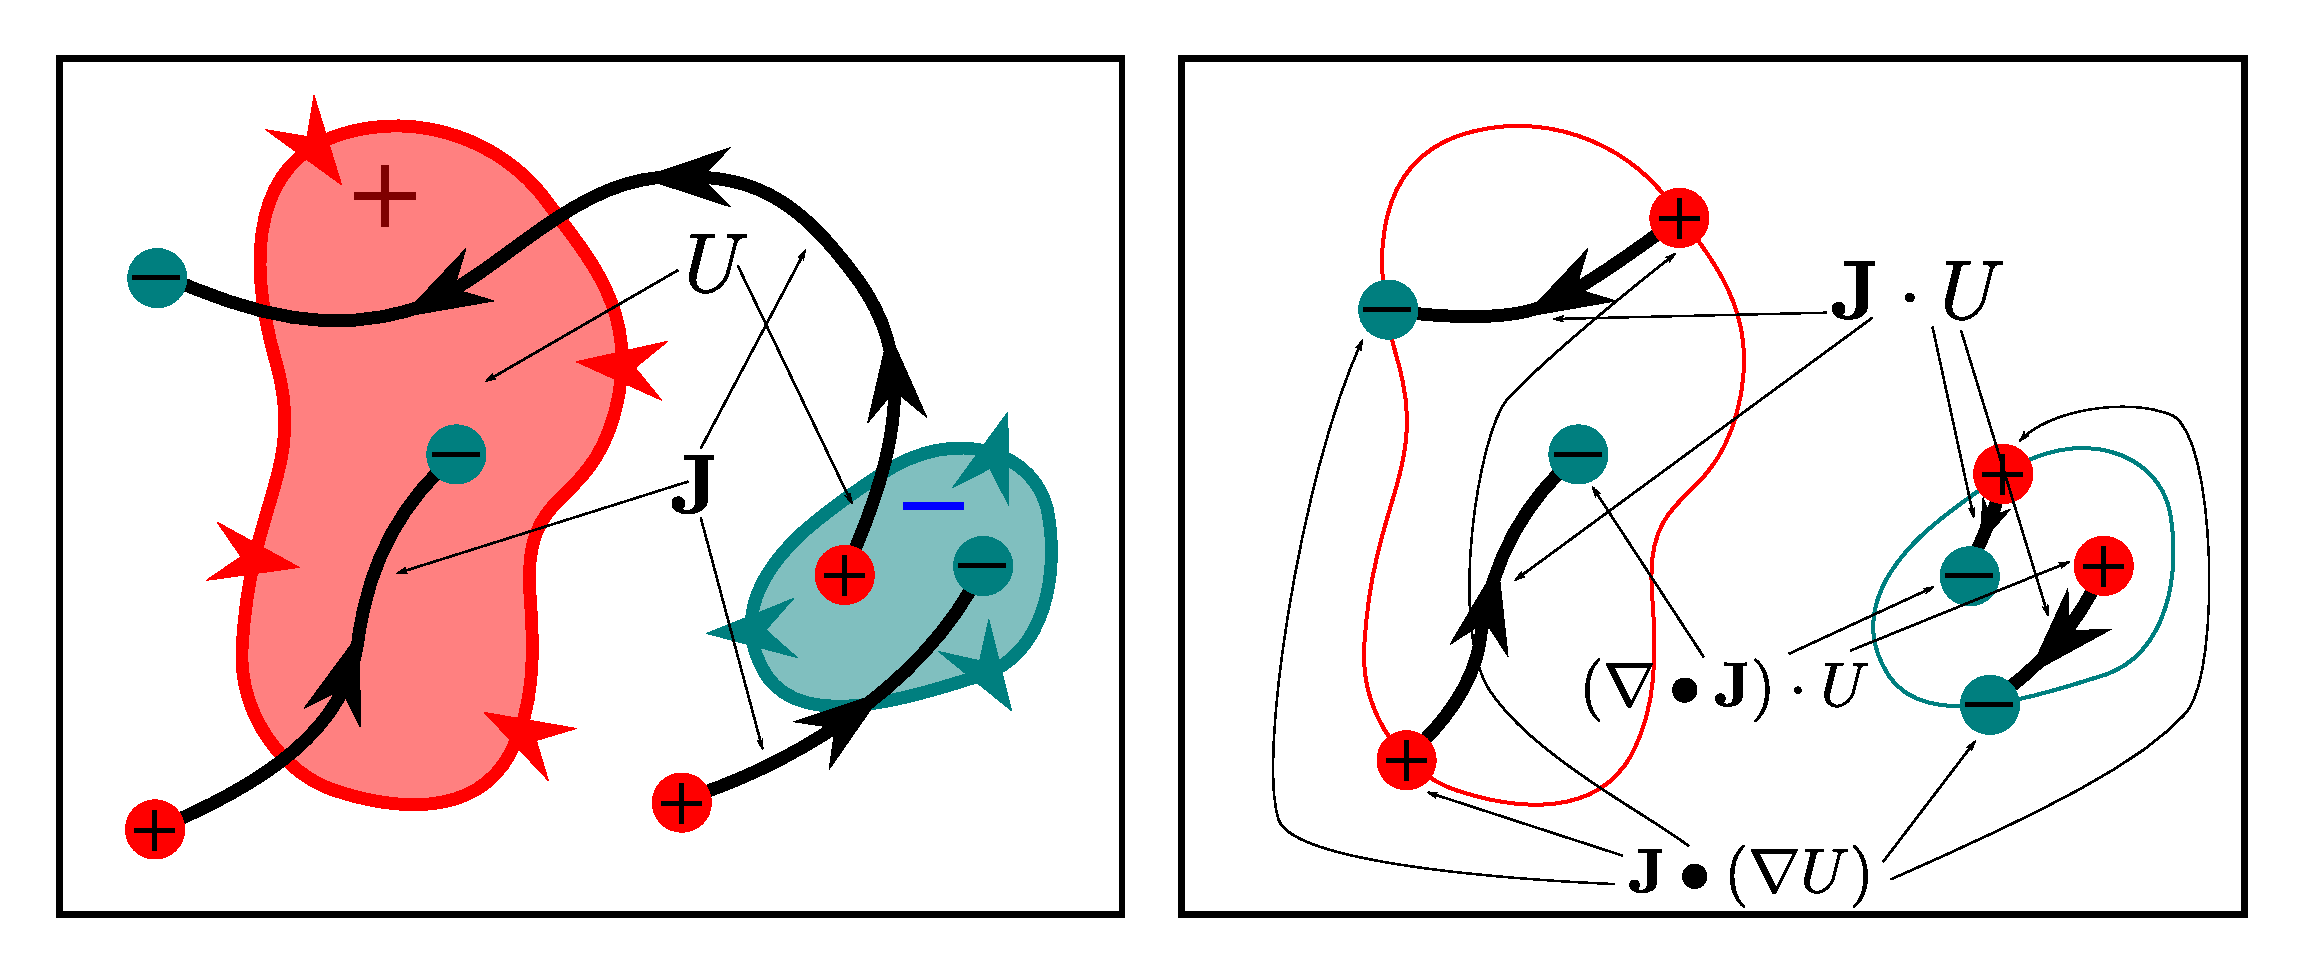
\includegraphics[width = 0.75\textwidth]{Boundaries/Path_endpoints/path_volume_intersection_endpoints}
\end{center}

\begin{center}
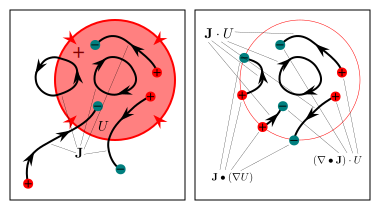
\includegraphics[width = 0.75\textwidth]{Boundaries/Path_endpoints/path_volume_intersection_endpoints_2}
\end{center}

Moreover, since the total endpoint weight is always \(0\), \(\int \nabla \bullet (\mathbf{J} \cdot U) = 0\) so \(\int ((\nabla \bullet \mathbf{J}) \cdot U + \mathbf{J} \bullet (\nabla U)) = 0\) so:

\begin{thm}
\[\int \mathbf{J} \bullet (\nabla U) = \int -(\nabla \bullet \mathbf{J}) \cdot U\]
\end{thm}

This statement reads that the net number of times path \(\mathbf{J}\) enters volume \(U\), {\bf where exits count against entrances}, is equal to the net number of finishing points left inside of \(U\), {\bf where starting points count against finishing points}. This statement is referred to as either the {\bf gradient theorem} or the {\bf divergence theorem}.

\begin{tabular}{cc}
\parbox{0.5\textwidth}{
In the example on the right, there is a multi-path \(\mathbf{J}\) (which consists of a single path) passing through a multi-volume \(U\). The total number of times \(\mathbf{J}\) enters \(U\) is: 
\[\int \mathbf{J} \bullet (\nabla U) = +1 - 1 - 1 + 1 + 1 + 1 - 1 + 1 + 1 + 1 = 4\] 
The total number of finishing points left in \(U\) is:
\[\int -(\nabla \bullet \mathbf{J}) \cdot U = +5 - 1 = 4\]
The \(+5\) comes from the fact that the finishing point sits inside \(5\) volumes, while the \(-1\) comes from the starting point sitting inside \(1\) volume.

It is clear that in this example:
 \[\int \mathbf{J} \bullet (\nabla U) = \int -(\nabla \bullet \mathbf{J}) \cdot U\]

} & \parbox{0.5\textwidth}{
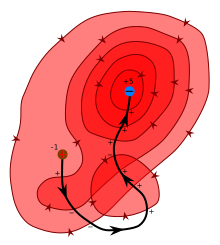
\includegraphics[width = 0.5\textwidth]{Boundaries/Path_endpoints/Gradient_theorem}
}
\end{tabular}

\begin{tabular}{cc}
\parbox{0.5\textwidth}{
In the next example on the right, there is a multi-path \(\mathbf{J}\) passing through a multi-volume \(U\) (which consists of a single volume). The total number of times \(\mathbf{J}\) enters \(U\) is: 
\[\int \mathbf{J} \bullet (\nabla U) = 5 \times (+1) + 8 \times (-1) = -3\] 
The total number of finishing points left in \(U\) is:
\[\int -(\nabla \bullet \mathbf{J}) \cdot U = 2 \times (+1) + 5 \times (-1) = -3\]

It is clear that in this example:
 \[\int \mathbf{J} \bullet (\nabla U) = \int -(\nabla \bullet \mathbf{J}) \cdot U\]

} & \parbox{0.5\textwidth}{
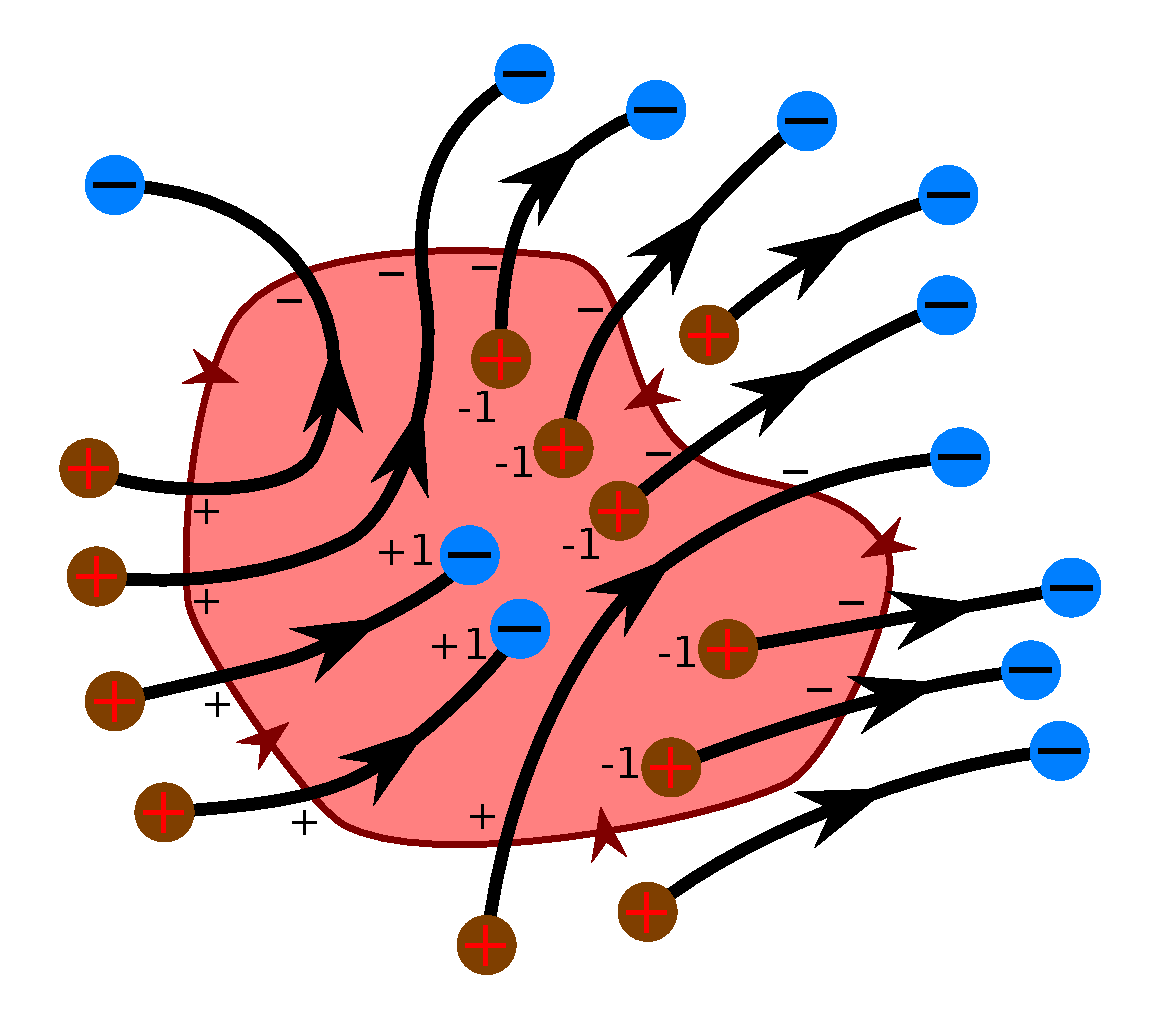
\includegraphics[width = 0.5\textwidth]{Boundaries/Path_endpoints/Divergence_theorem}
}
\end{tabular}




\section{The endpoints of surface-surface intersections}

Consider arbitrary multi-surfaces \(\mathbf{F}\) and \(\mathbf{G}\). The intersection \(\mathbf{F} \times \mathbf{G}\) is a multi-path, and the endpoints of this intersection are what will be sought: \(\nabla \bullet (\mathbf{F} \times \mathbf{G})\)

Endpoints of \(\mathbf{F} \times \mathbf{G}\) occur whenever a boundary of \(\mathbf{F}\) intersects \(\mathbf{G}\), or vice versa as depicted below. 

\begin{center}
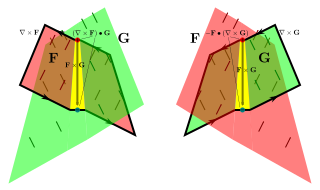
\includegraphics[width = 0.75\textwidth]{Boundaries/Path_endpoints/surface_surface_intersection_endpoints_2}
\end{center}

On the left, when the counterclockwise boundary of \(\mathbf{F}\) intersects \(\mathbf{G}\) in the preferred direction, starting points of \(\mathbf{F} \times \mathbf{G}\) are created, and when the counterclockwise boundary of \(\mathbf{F}\) intersects \(\mathbf{G}\) in the opposite direction, finishing points of \(\mathbf{F} \times \mathbf{G}\) are created. Therefore the intersection of the boundary of \(\mathbf{F}\) with the multi-surface \(\mathbf{G}\) contributes endpoints to \(\mathbf{F} \times \mathbf{G}\). This intersection is \((\nabla \times \mathbf{F}) \bullet \mathbf{G}\)

On the right, when the counterclockwise boundary of \(\mathbf{G}\) intersects \(\mathbf{F}\) in the preferred direction, finishing points of \(\mathbf{F} \times \mathbf{G}\) are created, and when the counterclockwise boundary of \(\mathbf{G}\) intersects \(\mathbf{F}\) in the opposite direction, starting points of \(\mathbf{F} \times \mathbf{G}\) are created. Therefore the intersection of the boundary of \(\mathbf{G}\) with the multi-surface \(\mathbf{F}\) contributes endpoints to \(\mathbf{F} \times \mathbf{G}\), but the {\bf polarity of the intersection points must be flipped to match the endpoints}. This intersection is \(-\mathbf{F} \bullet (\nabla \times \mathbf{G})\)

In total:
\begin{thm}
\[\nabla \bullet (\mathbf{F} \times \mathbf{G}) = (\nabla \times \mathbf{F}) \bullet \mathbf{G} - \mathbf{F} \bullet (\nabla \times \mathbf{G})\]
\end{thm}

Another example is depicted below, where both of the intersections \((\nabla \times \mathbf{F}) \bullet \mathbf{G}\) and \(\mathbf{F} \bullet (\nabla \times \mathbf{G})\) are nonzero. On the left, \(\mathbf{F}\) and \(\mathbf{G}\) are both depicted; along with their counterclockwise oriented boundaries \(\nabla \times \mathbf{F}\) and \(\nabla \times \mathbf{G}\); and also the intersections \((\nabla \times \mathbf{F}) \bullet \mathbf{G}\) and \(\mathbf{F} \bullet (\nabla \times \mathbf{G})\). On the right, the intersection \(\mathbf{F} \times \mathbf{G}\) is depicted along with the endpoints \(\nabla \bullet (\mathbf{F} \times \mathbf{G})\).

\begin{center}
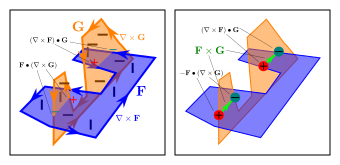
\includegraphics[width = 0.75\textwidth]{Boundaries/Path_endpoints/surface_surface_intersection_endpoints}
\end{center}

Moreover, since the total endpoint weight is always \(0\), \(\int \nabla \bullet (\mathbf{F} \times \mathbf{G}) = 0\) so \(\int ((\nabla \times \mathbf{F}) \bullet \mathbf{G} - \mathbf{F} \bullet (\nabla \times \mathbf{G})) = 0\) so:

\begin{thm}
\[\int (\nabla \times \mathbf{F}) \bullet \mathbf{G} = \int \mathbf{F} \bullet (\nabla \times \mathbf{G})\]
\end{thm}

This statement reads that the net number of times the counterclockwise boundary of \(\mathbf{F}\) passes throguh \(\mathbf{G}\), is equal to the net number of times that the counterclockwise boundary of \(\mathbf{G}\) passes throguh \(\mathbf{F}\). This statement is generally referred to as {\bf Stokes' Theorem}.

\begin{tabular}{cc}
\parbox{0.5\textwidth}{
If \(\mathbf{A}\) and \(\mathbf{B}\) are multi-loops, and \(\mathbf{F}\) and \(\mathbf{G}\) are multi-surfaces whose counter-clockwise boundaries are respectively \(\mathbf{A}\) and \(\mathbf{B}\), then:

\[\int \mathbf{A} \bullet \mathbf{G} = \int \mathbf{B} \bullet \mathbf{F}\]

\(\int \mathbf{A} \bullet \mathbf{G}\) is the number of times multi-loop \(\mathbf{A}\) loops through multi-loop \(\mathbf{B}\), while \(\int \mathbf{B} \bullet \mathbf{F}\) is the number of times multi-loop \(\mathbf{B}\) loops through multi-loop \(\mathbf{A}\).

In the image on the right, the two loops link through each other \(2\) times. 
} & \parbox{0.5\textwidth}{
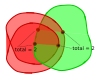
\includegraphics[width = 0.5\textwidth]{Boundaries/Path_endpoints/Stokes_theorem}
}
\end{tabular}




\section{The boundaries of surface-volume intersections}

Consider an arbitrary multi-surface \(\mathbf{F}\) and an arbitrary multi-volume \(U\). The intersection \(\mathbf{F} \cdot U\) is a multi-surface, and the counterclockwise boundary of this intersection is what will be sought: \(\nabla \times (\mathbf{F} \cdot U)\) 

Given an oriented surface \(\sigma\) and a volume \(\Omega\), there are two sources of boundaries for \(\sigma \cdot \Omega\). The sections of the boundaries of \(\sigma\) that happen to be inside of \(\Omega\) are also sections of the boundary of \(\sigma \cdot \Omega\). In addition, when \(\sigma\) slices into \(\Omega\), this also creates sections of the boundary for the intersection \(\sigma \cdot \Omega\).   

Consider a multi-surface \(\mathbf{F}\) and a multi-volume \(U\). The sections of the counterclockwise boundary of \(\mathbf{F}\) that are contained in \(U\), \((\nabla \times \mathbf{F}) \cdot U\), are sections of the counterclockwise boundary of \(\mathbf{F} \cdot U\). In addition, the intersection of the inwards oriented surface of \(U\) with \(\mathbf{F}\), \((\nabla U) \times \mathbf{F}\), also generates sections of the counterclockwise boundary for \(\mathbf{F} \cdot U\). The intersection \((\nabla U) \times \mathbf{F}\) has the correct orientation as opposed to \(\mathbf{F} \times (\nabla U)\), as illustrated below. In total,  

\begin{thm}
\[\nabla \times (\mathbf{F} \cdot U) = (\nabla \times \mathbf{F}) \cdot U + (\nabla U) \times \mathbf{F}\]
\end{thm}

\begin{tabular}{cc}
\parbox{0.5\textwidth}{
To the right, an example surface \(\mathbf{F}\) and volume \(U\) is shown, where \(\mathbf{F}\) is partially embedded in \(U\). The boundary of intersection \(\mathbf{F} \cdot U\) consists of two parts: 

The first part is the section of \(\nabla \times \mathbf{F}\) that is embedded in \(U\), \((\nabla \times \mathbf{F}) \cdot U\). 

The second part is the intersection of \(\mathbf{F}\) with the inwards oriented surface of \(U\) instead of with the inwards oriented surface of reality: \((\nabla U) \times \mathbf{F}\) instead of \(\nabla \times \mathbf{F}\).  
} & \parbox{0.5\textwidth}{
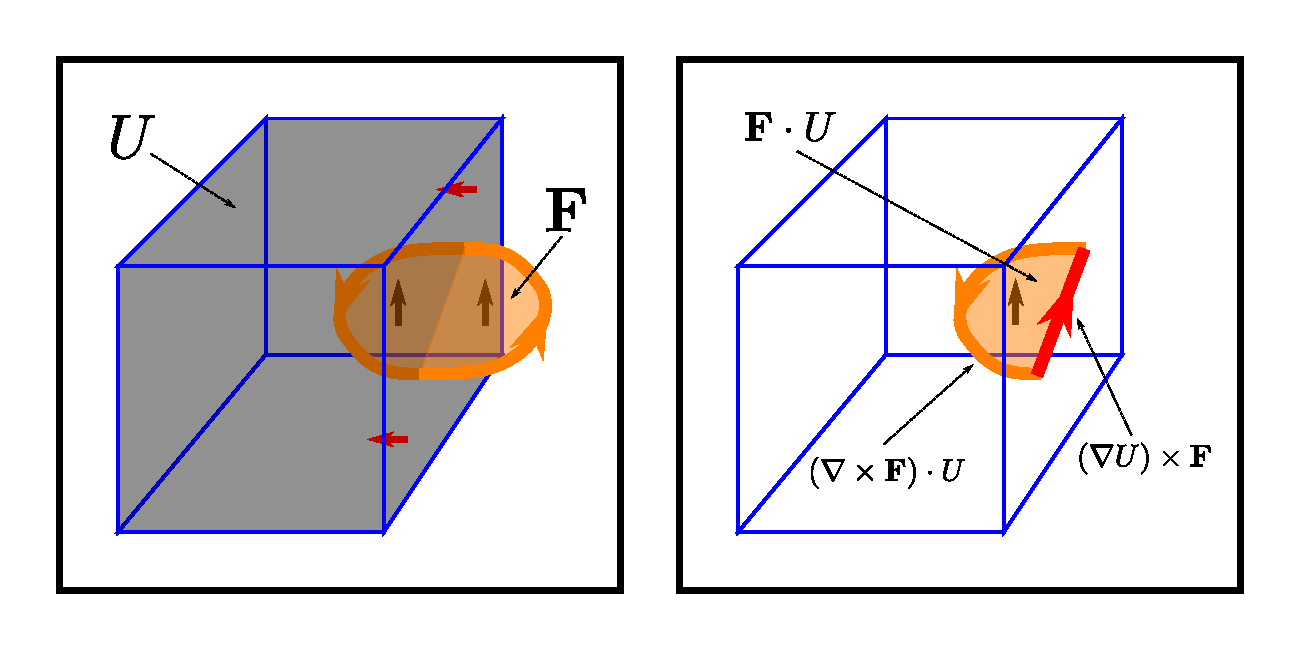
\includegraphics[width = 0.5\textwidth]{Boundaries/Surface_boundaries/surface_volume_intersection_boundary}
}
\end{tabular}

The ordering of the factors in the \(2^\text{nd}\) term \((\nabla U) \times \mathbf{F}\) can be easily remembered as opposed to \(\mathbf{F} \times (\nabla U)\) using the following mnemonic. In the second term \((\nabla U) \times \mathbf{F}\), the inwards oriented surface of \(U\), \(\nabla U\), replaces the inwards oriented surface of reality, \(\nabla\), in the expression \(\nabla \times \mathbf{F}\). In the image below, on the left is the boundary \(\nabla \times (\mathbf{F} \cdot U)\), and on the right is the intersection \((\nabla U) \times \mathbf{F}\).

\begin{center}
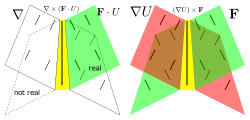
\includegraphics[width = 0.75\textwidth]{Boundaries/Surface_boundaries/surface_volume_intersection_mnemonic}
\end{center}




\section{The surfaces of volume-volume intersections}

Lastly, consider two multi-volumes \(U\) and \(V\). The intersection \(U \cdot V\) is a multi-volume, and the inwards-oriented surface of this intersection is what will be sought: \(\nabla(U \cdot V)\)

The surface of the intersection \(U \cdot V\) consists of the surface of \(U\) that is embedded in \(V\), plus the surface of \(V\) that is embedded in \(U\), as depicted below: 

\begin{thm}
\[\nabla(U \cdot V) = (\nabla U) \cdot V + U \cdot (\nabla V)\]
\end{thm}

\begin{center}
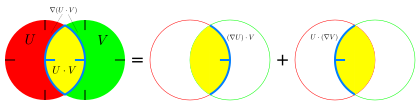
\includegraphics[width = \textwidth]{Boundaries/Volume_inwards_oriented_surfaces/volume_volume_intersection_surface}
\end{center}



\section{Summary}

To summarize the boundaries of the various intersections, 

\begin{center}
\begin{tabular}{|c|c||c|c|}
\hline
multi-structure 1 
& multi-structure 2 
& intersection 
& intersection boundary 
\\
\hline
\hline
point \(\rho\) 
& volume \(U\)
& point \(\rho \cdot U\) 
& N/A 
\\  
\hline
path \(\mathbf{J}\) 
& surface \(\mathbf{F}\) 
& point \(\mathbf{J} \bullet \mathbf{F}\)
& N/A
\\
\hline
path \(\mathbf{J}\) 
& volume \(U\) 
& path \(\mathbf{J} \cdot U\) 
& point \(\nabla \bullet (\mathbf{J} \cdot U) = (\nabla \bullet \mathbf{J}) \cdot U + \mathbf{J} \bullet (\nabla U)\) 
\\
\hline
surface \(\mathbf{F}\) 
& surface \(\mathbf{G}\) 
& path \(\mathbf{F} \times \mathbf{G}\) 
& point \(\nabla \bullet (\mathbf{F} \times \mathbf{G}) = (\nabla \times \mathbf{F}) \bullet \mathbf{G} - \mathbf{F} \bullet (\nabla \times \mathbf{G})\) 
\\
\hline
surface \(\mathbf{F}\)
& volume \(U\) 
& surface \(\mathbf{F} \cdot U\) 
& path \(\nabla \times (\mathbf{F} \cdot U) = (\nabla \times \mathbf{F}) \cdot U + (\nabla U) \times \mathbf{F}\)
\\
\hline
volume \(U\) 
& volume \(V\) 
& volume \(U \cdot V\) 
& surface \(\nabla (U \cdot V) = (\nabla U) \cdot V + U \cdot (\nabla V)\)
\\
\hline 
\end{tabular}
\end{center}

In addition it was observed that:

Given an arbitrary multi-path \(\mathbf{J}\) and an arbitrary multi-volume \(U\), then 
\[\int \mathbf{J} \bullet (\nabla U) = - \int (\nabla \bullet J) \cdot U\]

Given multi-surfaces \(\mathbf{F}\) and \(\mathbf{G}\), then
\[\int (\nabla \times \mathbf{F}) \bullet \mathbf{G} = \int \mathbf{F} \bullet (\nabla \times \mathbf{G})\]
(this is {\bf Stokes' theorem})


